\chapter{Transformada de \emph{Laplace}}

Dada una función $f(t)$ definida para $t>0$:
\begin{equation}
    \mathcal{L}\{f(t)\}=F(s)=\int_0^{\infty}f(t)\,e^{-st}\,dt
\end{equation}

Donde: $s=\sigma+j\omega$ es una frecuencia compleja.

La transformada de \emph{Laplace} convierte una función del dominio de ``t'' al
dominio de ``s''.

\section{Transformadas de funciones elementales}

\subsection{$k$}
\begin{equation*}
\begin{split}
    \mathcal{L}\{k\}
        &=\int_{0}^{\infty}k\,e^{-st}\,dt\\
        &=\frac{k\,e^{-st}}{-s}\Biggr|_0^{\infty}\\
        &=\frac{k}{-s}(0-1)\\
\end{split}
\end{equation*}
\begin{equation}
    \mathcal{L}\{k\}=\frac{k}{s}
\end{equation}

\subsection{$t^n\quad\,\in\mathbb{N}$}
Para $n=1$:
\begin{equation*}
\begin{split}
    \mathcal{L}\{t\}
        &=\int_0^{\infty}t\,e^{-st}\,dt\\
        &=\left(\frac{t\,e^{-st}}{-s}\Biggr|_0^{\infty}\right)
        -\left(\frac{e^{-st}}{{(-s)}^2}\Biggr|_0^{\infty}\right)\\
        &=\frac{-0-1}{{(-s)}^2}\\
        &=\frac{1}{s^2}
\end{split}
\end{equation*}

Para $n=2$:
\begin{equation*}
\begin{split}
    \mathcal{L}\{t^2\}
        &=\int_0^{\infty}t^2\,e^{-st}\,dt\\
\end{split}
\end{equation*}
\begin{equation*}
    u=t^2
\end{equation*}
\begin{equation*}
    du=2t\,dt
\end{equation*}
\begin{equation*}
    dv=e^{-st}\,dt
\end{equation*}
\begin{equation*}
    v=\frac{e^{-st}}{-s}
\end{equation*}
\begin{equation*}
\begin{split}
    \mathcal{L}\{t^2\}
        &=\int_0^{\infty}t^2\,e^{-st}\,dt\\
        &=\left(\frac{t^2\,e^{-st}}{-s}\Biggr|_0^{\infty}\right)
        -\int_0^{\infty}\frac{e^{-st}}{-s}\,2t\,dt\\
        &=\frac{2}{s}\int_0^{\infty}t\,e^{-st}\,dt\\
        &=\frac{2}{s}\left(\frac{1}{s^2}\right)\\
        &=\frac{2}{s^3}
\end{split}
\end{equation*}

Para $n=3$:
\begin{equation*}
\begin{split}
    \mathcal{L}\{t^3\}
        &=\int_0^{\infty}t^3\,e^{-st}\,dt\\
\end{split}
\end{equation*}
\begin{equation*}
    u=t^3
\end{equation*}
\begin{equation*}
    du=3t^2\,dt
\end{equation*}
\begin{equation*}
    dv=e^{-st}\,dt
\end{equation*}
\begin{equation*}
    v=\frac{e^{-st}}{-s}
\end{equation*}
\begin{equation*}
\begin{split}
    \mathcal{L}\{t^3\}
        &=\int_0^{\infty}t^3\,e^{-st}\,dt\\
        &=\left(\frac{t^3\,e^{-st}}{-s}\Biggr|_0^{\infty}\right)
        -\int_0^{\infty}\frac{e^{-st}}{-s}\,3t^2\,dt\\
        &=\frac{3}{s}\int_0^{\infty}t^2\,e^{-st}\,dt\\
        &=\frac{3}{s}\left(\frac{2}{s^3}\right)\\
        &=\frac{6}{s^4}
\end{split}
\end{equation*}

\begin{equation}
    \mathcal{L}\{t^n\}=\frac{n!}{s^{n+1}}
\end{equation}

\subsection{$e^{at}$}
\begin{equation*}
\begin{split}
    \mathcal{L}\{e^{at}\}
        &=\int_0^{\infty}e^{at}\,e^{-st}\,dt\\
        &=\int_0^{\infty}e^{-(s-a)t}\,dt\\
        &=\left(\frac{e^{-(s-a)t}}{-(s-a)}\Biggr|_0^{\infty}\right)\\
        &=\frac{0-1}{-(s-a)}
\end{split}
\end{equation*}

\begin{equation}
    \mathcal{L}\{e^{at}\}=\frac{1}{s-a}
\end{equation}

\subsection{$\sen(at)$}
\begin{equation*}
\begin{split}
    \mathcal{L}\{\sen(at)\}
        &=\mathcal{L}\biggl\{\frac{e^{jat}-e^{-jat}}{2j}\biggl\}\\
        &=\frac{1}{2j}\left(\frac{1}{s-ja}-\frac{1}{s+ja}\right)\\
        &=\frac{1}{2j}\left(\frac{s+ja-s+ja}{(s-ja)(s+ja)}\right)
\end{split}
\end{equation*}

\begin{equation}
    \mathcal{L}\{\sen(at)\}=\frac{a}{s^2+a^2}
\end{equation}

\subsection{$\cos(at)$}
\begin{equation*}
\begin{split}
    \mathcal{L}\{\cos(at)\}
        &=\mathcal{L}\biggl\{\frac{e^{jat}+e^{-jat}}{2}\biggl\}\\
        &=\frac{1}{2}\left(\frac{1}{s-ja}-\frac{1}{s+ja}\right)\\
        &=\frac{1}{2}\left(\frac{s+ja+s-ja}{(s-ja)(s+ja)}\right)
\end{split}
\end{equation*}

\begin{equation}
    \mathcal{L}\{\cos(at)\}=\frac{s}{s^2+a^2}
\end{equation}

\subsection{$\senh(at)$}
\begin{equation*}
\begin{split}
    \mathcal{L}\{\senh(at)\}
        &=\mathcal{L}\biggl\{\frac{e^{at}-e^{-at}}{2}\biggl\}\\
        &=\frac{1}{2}\left(\frac{1}{s-a}-\frac{1}{s+a}\right)\\
        &=\frac{1}{2}\left(\frac{s+a-s+a}{(s-a)(s+a)}\right)
\end{split}
\end{equation*}

\begin{equation}
    \mathcal{L}\{\senh(at)\}=\frac{a}{s^2-a^2}
\end{equation}

\subsection{$\cosh(at)$}
\begin{equation*}
\begin{split}
    \mathcal{L}\{\cosh(at)\}
        &=\mathcal{L}\biggl\{\frac{e^{at}+e^{-at}}{2}\biggl\}\\
        &=\frac{1}{2}\left(\frac{1}{s-a}-\frac{1}{s+a}\right)\\
        &=\frac{1}{2}\left(\frac{s+a+s-a}{(s-ja)(s+ja)}\right)
\end{split}
\end{equation*}

\begin{equation}
    \mathcal{L}\{\cosh(at)\}=\frac{s}{s^2-a^2}
\end{equation}

\section{Propiedades de la transformada de \emph{Laplace}}

\subsection{Linealidad}
\begin{equation}
    \mathcal{L}\{a_1f_1(t)+a_2f_2(t)\}=a_1F_1(s)+a_2F_2(s)
\end{equation}

\subsection{Desplazamiento en $s$}
Si $\mathcal{L}\{f(t)\}=F(s)$:
\begin{equation}
    \mathcal{L}\{f(t)\,e^{at}\}=F(s-a)
\end{equation}

\subsection{Desplazamiento en $t$}
Si $\mathcal{L}\{f(t)\}=F(s)$:
\begin{equation}
    \mathcal{L}\{f(t-a)\,u(t-a)\}=F(s)\,e^{-as}
\end{equation}

$f(t)$ esta definida para $t>0$, por tanto: $f(t)=f(t)\,u(t)$.

Segunda forma:
\begin{equation*}
\begin{split}
    \mathcal{L}\{f(t)\,u(t-a)\}
        &=\int_a^{\infty}f(t)\,e^{-st}\,dt
\end{split}
\end{equation*}
\begin{equation*}
    \tau=t-a\,\rightarrow\,t=\tau+a
\end{equation*}
\begin{equation*}
    d\tau=dt
\end{equation*}
\begin{equation*}
\begin{split}
    \mathcal{L}\{f(t)\,u(t-a)\}
        &=\int_0^{\infty}f(\tau+a)\,e^{-s(\tau+a)}\,dt\\
        &=e^{-as}\int_0^{\infty}f(\tau+a)\,e^{-st}\,d\tau\\
\end{split}
\end{equation*}
\begin{equation}
    \mathcal{L}\{f(t)\,u(t-a)\}=e^{-as}\mathcal{L}\{f(t+a)\}
\end{equation}

\subsection{Multiplicación por $t$}
Si $\mathcal{L}\{f(t)\}=F(s)$:
\begin{equation}
    \mathcal{L}\{t\,f(t)\}=-\frac{dF(s)}{ds}
\end{equation}
\begin{equation}
    \mathcal{L}\{t^n\,f(t)\}={(-1)}^n\frac{d^{(n)}F(s)}{ds^n}
\end{equation}

\subsection{División por $t$}
Si $\mathcal{L}\{f(t)\}=F(s)$:
\begin{equation}
    \mathcal{L}\biggl\{\frac{1}{t}f(t)\biggl\}=\int_s^{\infty}F(s)\,ds
\end{equation}

\underline{Prueba}:

\begin{equation*}
    g(t)=\frac{1}{t}f(t)\,\rightarrow\,f(t)=t\,g(t)
\end{equation*}
\begin{equation*}
    \mathcal{L}\{f(t)\}=\mathcal{L}\{t\,g(t)\}\\
\end{equation*}
\begin{equation*}
    F(s)=-\frac{dG(s)}{ds}
\end{equation*}
\begin{equation*}
    \int_s^{\infty}dG(s)=\int_s^{\infty}-dF(s)\,ds
\end{equation*}
\begin{equation*}
    G(\infty)-G(s)=-\int_s^{\infty}F(s)\,ds
\end{equation*}

Asumiendo que $G(\infty)=0$:
\begin{equation*}
    G(s)=\int_s^{\infty}F(s)\,ds
\end{equation*}
\begin{equation*}
    \mathcal{L}\biggl\{\frac{1}{t}f(t)\biggl\}=\int_s^{\infty}F(s)\,ds
\end{equation*}

\textbf{Ejemplo}:
\begin{equation*}
    \mathcal{L}\biggl\{\frac{1}{t}sen(at)\biggl\}
\end{equation*}
\begin{equation*}
\begin{split}
    \mathcal{L}\biggl\{\frac{1}{t}sen(at)\biggl\}
        &=\int_s^{\infty}\frac{a}{s^2+a^2}\,ds\\
        &=\arctan\left(\frac{s}{a}\right)\Biggr|_s^{\infty}\\
        &=\frac{\pi}{2}-\arctan\left(\frac{s}{a}\right)
\end{split}
\end{equation*}
\begin{equation*}
    u=\frac{\pi}{2}-\arctan\left(\frac{s}{a}\right)
    \rightarrow
    \arctan\left(\frac{s}{a}\right)=\frac{\pi}{2}-u
    \rightarrow
    \tan\left(\frac{\pi}{2}-u\right)=\frac{s}{a}
\end{equation*}
\begin{equation*}
    \tan(u)=\frac{a}{s}
    \rightarrow
    u=\arctan\left(\frac{a}{s}\right)
\end{equation*}
\begin{equation*}
    \mathcal{L}\biggl\{\frac{1}{t}sen(at)\biggl\}
        =\arctan\left(\frac{a}{s}\right)
\end{equation*}

\section{Tabla de transformadas de \emph{Laplace}}

\begin{equation*}
\def\arraystretch{1.4}
\begin{array}{@{}cll@{}}
\toprule
 & f(t) & F(s)=\mathcal{L}\{f(t)\}\\
\cmidrule(l){2-3}
 1 & k
   & \dfrac{k}{s}\\
\cmidrule(l){2-3}
 2 & t^n
   & \dfrac{n!}{s^{n+1}}\quad\,n\in\mathbb{N}\\
\cmidrule(l){2-3}
 3 & e^{at}
   & \dfrac{1}{s-a}\\
\cmidrule(l){2-3}
 4 & \sen(at)
   & \dfrac{a}{s^2+a^2}\\
\cmidrule(l){2-3}
 5 & \cos(at)
   & \dfrac{s}{s^2+a^2}\\
\cmidrule(l){2-3}
 6 & \senh(at)
   & \dfrac{a}{s^2-a^2}\\
\cmidrule(l){2-3}
 7 & \cosh(at)
   & \dfrac{s}{s^2-a^2}\\
\cmidrule(l){2-3}
 8 & u(t-a)
   & \dfrac{1}{s}e^{-as}\\
\cmidrule(l){2-3}
 9 & \delta(t-a)
   & e^{-at}\\
\cmidrule(l){2-3}
10 & \dfrac{1}{t}\sen(at)
   & \arctan\left(\dfrac{a}{s}\right)\\
\bottomrule
\end{array}
\end{equation*}

\section{Transformada de \emph{Laplace} de derivadas}
Si $\mathcal{L}\{f(t)\}=F(s)$, las transformadas de sus derivadas serán:

\begin{equation}
    \mathcal{L}\{f'(t)\}=sF(s)-f(0)
\end{equation}
\begin{equation}
    \mathcal{L}\{f''(t)\}=s^2F(s)-f(0)s-f'(0)
\end{equation}
\begin{equation}
    \mathcal{L}\{f^{\prime\prime\prime}(t)\}=s^3F(s)-f(0)s^2-f'(0)s-f''(0)
\end{equation}

En general, de una derivada n-ésima:
\begin{equation}
    \mathcal{L}\{f^{(n)}(t)\}=s^{n}F(s)-f(0)s^{n-1}-f'(0)s^{n-2}-f''(0)s^{n-3}
    -\cdots-f^{(n-1)}(0)
\end{equation}

Donde: $f(0);f'(0);f''(0);\ldots;f^{(n-1)}(0)$ son los valores iniciales en
$t=0$ de la función y de sus derivadas.

\underline{Prueba}:

\begin{equation*}
    \mathcal{L}\{f'(t)\}=\int_0^{\infty}f'(t)\,e^{-st}\,dt
\end{equation*}
\begin{equation*}
    u=e^{-st}
\end{equation*}
\begin{equation*}
    du=-s\,e^{-st}\,dt
\end{equation*}
\begin{equation*}
    dv=f'(t)\,dt
\end{equation*}
\begin{equation*}
    v=f(t)
\end{equation*}
\begin{equation*}
\begin{split}
    \mathcal{L}\{f'(t)\}
        &=(f(t)\,e^{-st}\Biggr|_0^{\infty})
        -\int_0^{\infty}f(t)(-s\,e^{-st})\,dt\\
        &=s\int_0^{\infty}f(t)\,e^{-st}\,dt-f(0)\\
        &=sF(s)-f(0)
\end{split}
\end{equation*}
\begin{equation*}
\begin{split}
    \mathcal{L}\{f''(t)\}
        &=s\mathcal{L}\{f'(t)\}-f'(0)\\
        &=s(sF(s)-f(0))-f'(0)\\
        &=s^2F(s)-f(0)s-f'(0)
\end{split}
\end{equation*}
\begin{equation*}
\begin{split}
    \mathcal{L}\{f\prime\prime\prime(t)\}
        &=s\mathcal{L}\{f''(t)\}-f''(0)\\
        &=s(s^2F(s)-f(0)s-f'(0))-f''(0)\\
        &=s^3F(s)-f(0)s^2-f'(0)s-f''(0)
\end{split}
\end{equation*}

\section{Transformada de \emph{Laplace} de integrales}
Si $\mathcal{L}\{f(t)\}=F(s)$:

\begin{equation}
    \mathcal{L}\biggl\{\int_0^t\,f(t)\,dt\biggl\}=\frac{1}{s}F(s)
\end{equation}

\underline{Prueba}:

\begin{equation*}
    g(t)=\int_0^t\,f(t)\,dt\rightarrow\,g'(t)=f(t)
\end{equation*}
\begin{equation*}
    \mathcal{L}\{g'(t)\}=\mathcal{L}\{f(t)\}\\
\end{equation*}
\begin{equation*}
    sG(s)-g(0)=F(s)
\end{equation*}
\begin{equation*}
    s\mathcal{L}\{\biggl\{\int_0^t\,f(t)\,dt\biggl\}=F(s)
\end{equation*}
\begin{equation*}
    \mathcal{L}\biggl\{\int_0^t\,f(t)\,dt\biggl\}=\frac{1}{s}F(s)
\end{equation*}

\section{La función \emph{Gamma}}
\begin{equation}
    \Gamma(n)=\int_0^{\infty}\,x^{n-1}\,e^{-x}\,dx
\end{equation}

\subsection{Propiedades de la función \emph{Gamma}}

\subsubsection*{Propiedad 1}
\begin{equation}
    \Gamma(n)=(n-1)\Gamma(n-1)
\end{equation}

En general:
\begin{equation}
    \Gamma(n)=(n-1)(n-2)(n-3)\dots(n-r)\Gamma(n-r)
\end{equation}

\underline{Prueba}:

\begin{equation*}
    \Gamma(n)=\int_0^{\infty}\,x^{n-1}\,e^{-x}\,dx
\end{equation*}
\begin{equation*}
    u=x^{n-1}
\end{equation*}
\begin{equation*}
    du=(n-1)\,x^{n-2}\,dx
\end{equation*}
\begin{equation*}
    dv=e^{-x}\,dx
\end{equation*}
\begin{equation*}
    v=-e^{-x}
\end{equation*}
\begin{equation*}
\begin{split}
    \Gamma(n)
        &=(-x^{n-1}\,e^{-x}\Bigg|_0^{\infty})
        -\int_0^{\infty}-e^{-x}(n-1)x^{n-2}\,dx\\
        &=(n-1)\int_0^{\infty}\,x^{(n-1)-1}\,e^{-x}\,dx\\
        &=(n-1)\Gamma(n-1)
\end{split}
\end{equation*}
\begin{equation*}
    \Gamma(n-1)=(n-2)\Gamma(n-2)
\end{equation*}
\begin{equation*}
    \Gamma(n-2)=(n-3)\Gamma(n-3)
\end{equation*}
\begin{equation*}
    \Gamma(n)=(n-1)(n-2)(n-3)\dots(n-r)\Gamma(n-r)
\end{equation*}

\subsubsection*{Propiedad 2}
\begin{equation}
    \Gamma(n)=\frac{\Gamma(n+1)}{n}
\end{equation}

\underline{Prueba}:

\begin{equation*}
    \Gamma(n)=(n-1)\Gamma(n-1)
\end{equation*}
\begin{equation*}
    \Gamma(n+1)=n\Gamma(n)
\end{equation*}
\begin{equation*}
    \Gamma(n)=\frac{1}{n}\Gamma(n+1)
\end{equation*}

\subsubsection*{Propiedad 3}
Si $n\in\mathbb{N}$:

\begin{equation}
    \Gamma(n)=(n-1)!
\end{equation}
\begin{equation}
    \Gamma(n+1)=n!
\end{equation}

\underline{Prueba}:

\begin{equation*}
    \Gamma(n)=(n-1)(n-2)(n-3)\dots(3)(2)(1)\,\Gamma(1)
\end{equation*}
\begin{equation*}
\begin{split}
    \Gamma(1)
        &=\int_0^{\infty}x^{1-1}\,e^{-x}\,dx\\
        &=-e^{-x}\Biggr|_0^{\infty}\\
        &=-(0-1)\\
        &=1
\end{split}
\end{equation*}

En particular $n=1$:

\begin{equation*}
    \Gamma(1)=(1-1)!
\end{equation*}
\begin{equation*}
    \Gamma(1)=0!
\end{equation*}
\begin{equation}
    1=0!
\end{equation}

\section{Evaluación de la función \emph{Gamma}}
Dada la integral:

\begin{equation*}
    I=\int_0^{\infty}e^{-x^2}\,dx
\end{equation*}
\begin{equation*}
    I=\int_0^{\infty}e^{-y^2}\,dy
\end{equation*}
\begin{equation*}
    I^2=\int_0^{\infty}e^{-x^2}\,dx\,\int_0^{\infty}e^{-y^2}\,dy
        =\int_0^{\infty}\int_0^{\infty}e^{-(x^2+y^2)}\,dy\,dx
\end{equation*}

Transformando a coordenadas polares:
\begin{equation*}
    x^2+y^2=r^2
\end{equation*}
\begin{equation*}
    dx\,dy=r\,dr\,d\theta
\end{equation*}

Por tanto:
\begin{equation*}
    I^2=\lim_{M\rightarrow\infty}\int_0^{\frac{\pi}{2}}
        \int_0^{M}e^{-r^2}r\,dr\,d\theta
\end{equation*}
\begin{equation*}
    u=-r^2
\end{equation*}
\begin{equation*}
    du=-2r\,dr
\end{equation*}
\begin{equation*}
\begin{split}
    I^2
        &=\lim_{M\rightarrow\infty}\int_0^{\frac{\pi}{2}}d\theta
        \int_0^{M}e^u\left(\frac{-dt}{2}\right)\\
        &=\lim_{M\rightarrow\infty}\int_0^{\frac{\pi}{2}}d\theta
        \left(-\frac{e^{-r^2}}{2}\Biggr|_0^M\right)\\
        &=-\frac{1}{2}\int_0^{\frac{\pi}{2}}d\theta(0-1)\\
        &=\frac{1}{2}\frac{\pi}{2}\\
        &=\frac{\pi}{4}
\end{split}
\end{equation*}
\begin{equation*}
    I=\int_0^{\infty}e^{-x^2}\,dx=\frac{\sqrt{\pi}}{2}
\end{equation*}

\begin{equation*}
    \Gamma\left(\frac{1}{2}\right)=\int_0^{\infty}x^{-\frac{1}{2}}e^{-x}\,dx
\end{equation*}
\begin{equation*}
    x=u^2
\end{equation*}
\begin{equation*}
    dx=2u\,du
\end{equation*}
\begin{equation*}
\begin{split}
    \Gamma\left(\frac{1}{2}\right)
        &=\int_0^{\infty}{({u^2})}^{-\frac{1}{2}}e^{-u^2}\,2u\,du\\
        &=2\int_0^{\infty}e^{-u^2}\,du\\
        &=2\frac{\sqrt{\pi}}{2}\\
        &=\sqrt{\pi}
\end{split}
\end{equation*}

\begin{equation}
    \Gamma\left(\frac{1}{2}\right)=\sqrt{\pi}
\end{equation}

\begin{equation*}
    \Gamma\left(-\frac{1}{2}\right)
        =\frac{\Gamma(\frac{1}{2})}{-\frac{1}{2}}
        =\frac{\sqrt{\pi}}{-\frac{1}{2}}
        =-2\sqrt{\pi}
\end{equation*}
\begin{equation}
    \Gamma\left(-\frac{1}{2}\right)=-2\sqrt{\pi}
\end{equation}

\section{Transformada de \emph{Laplace} con la función \emph{Gamma}}

\begin{equation*}
    \mathcal{L}\{t^n\}=\int_0^{\infty}t^n\,e^{-st}\,dt
\end{equation*}
\begin{equation*}
    u=st\rightarrow\,t=\frac{u}{s}
\end{equation*}
\begin{equation*}
    du=s\,dt
\end{equation*}
\begin{equation*}
\begin{split}
    \mathcal{L}\{t^n\}
        &=\int_0^{\infty}{\left(\frac{u}{s}\right)}^n\,e^{-u}\,\frac{du}{s}\\
        &=\frac{1}{s^{n+1}}\int_0^{\infty}u^n\,e^{-u}\,du\\
        &=\frac{\Gamma(n+1)}{s^{n+1}}
\end{split}
\end{equation*}

\begin{equation}
    \mathcal{L}\{t^n\}=\frac{\Gamma(n+1)}{s^{n+1}}
\end{equation}

En particular para $n\in\mathbb{N}$:

\begin{equation}
    \mathcal{L}\{t^n\}=\frac{n!}{s^{n+1}}
\end{equation}

\section{Teoremas del valor inicial y final}

\begin{figure}[H]
    \centering
    % GNUPLOT: LaTeX picture with Postscript
\begingroup
  \makeatletter
  \providecommand\color[2][]{%
    \GenericError{(gnuplot) \space\space\space\@spaces}{%
      Package color not loaded in conjunction with
      terminal option `colourtext'%
    }{See the gnuplot documentation for explanation.%
    }{Either use 'blacktext' in gnuplot or load the package
      color.sty in LaTeX.}%
    \renewcommand\color[2][]{}%
  }%
  \providecommand\includegraphics[2][]{%
    \GenericError{(gnuplot) \space\space\space\@spaces}{%
      Package graphicx or graphics not loaded%
    }{See the gnuplot documentation for explanation.%
    }{The gnuplot epslatex terminal needs graphicx.sty or graphics.sty.}%
    \renewcommand\includegraphics[2][]{}%
  }%
  \providecommand\rotatebox[2]{#2}%
  \@ifundefined{ifGPcolor}{%
    \newif\ifGPcolor
    \GPcolorfalse
  }{}%
  \@ifundefined{ifGPblacktext}{%
    \newif\ifGPblacktext
    \GPblacktexttrue
  }{}%
  % define a \g@addto@macro without @ in the name:
  \let\gplgaddtomacro\g@addto@macro
  % define empty templates for all commands taking text:
  \gdef\gplbacktext{}%
  \gdef\gplfronttext{}%
  \makeatother
  \ifGPblacktext
    % no textcolor at all
    \def\colorrgb#1{}%
    \def\colorgray#1{}%
  \else
    % gray or color?
    \ifGPcolor
      \def\colorrgb#1{\color[rgb]{#1}}%
      \def\colorgray#1{\color[gray]{#1}}%
      \expandafter\def\csname LTw\endcsname{\color{white}}%
      \expandafter\def\csname LTb\endcsname{\color{black}}%
      \expandafter\def\csname LTa\endcsname{\color{black}}%
      \expandafter\def\csname LT0\endcsname{\color[rgb]{1,0,0}}%
      \expandafter\def\csname LT1\endcsname{\color[rgb]{0,1,0}}%
      \expandafter\def\csname LT2\endcsname{\color[rgb]{0,0,1}}%
      \expandafter\def\csname LT3\endcsname{\color[rgb]{1,0,1}}%
      \expandafter\def\csname LT4\endcsname{\color[rgb]{0,1,1}}%
      \expandafter\def\csname LT5\endcsname{\color[rgb]{1,1,0}}%
      \expandafter\def\csname LT6\endcsname{\color[rgb]{0,0,0}}%
      \expandafter\def\csname LT7\endcsname{\color[rgb]{1,0.3,0}}%
      \expandafter\def\csname LT8\endcsname{\color[rgb]{0.5,0.5,0.5}}%
    \else
      % gray
      \def\colorrgb#1{\color{black}}%
      \def\colorgray#1{\color[gray]{#1}}%
      \expandafter\def\csname LTw\endcsname{\color{white}}%
      \expandafter\def\csname LTb\endcsname{\color{black}}%
      \expandafter\def\csname LTa\endcsname{\color{black}}%
      \expandafter\def\csname LT0\endcsname{\color{black}}%
      \expandafter\def\csname LT1\endcsname{\color{black}}%
      \expandafter\def\csname LT2\endcsname{\color{black}}%
      \expandafter\def\csname LT3\endcsname{\color{black}}%
      \expandafter\def\csname LT4\endcsname{\color{black}}%
      \expandafter\def\csname LT5\endcsname{\color{black}}%
      \expandafter\def\csname LT6\endcsname{\color{black}}%
      \expandafter\def\csname LT7\endcsname{\color{black}}%
      \expandafter\def\csname LT8\endcsname{\color{black}}%
    \fi
  \fi
    \setlength{\unitlength}{0.0500bp}%
    \ifx\gptboxheight\undefined%
      \newlength{\gptboxheight}%
      \newlength{\gptboxwidth}%
      \newsavebox{\gptboxtext}%
    \fi%
    \setlength{\fboxrule}{0.5pt}%
    \setlength{\fboxsep}{1pt}%
    \definecolor{tbcol}{rgb}{1,1,1}%
\begin{picture}(5760.00,2880.00)%
    \gplgaddtomacro\gplbacktext{%
      \csname LTb\endcsname%%
      \put(393,824){\makebox(0,0)[r]{\strut{}}}%
      \put(393,2087){\makebox(0,0)[r]{\strut{}}}%
      \put(489,601){\makebox(0,0){\strut{}}}%
      \put(987,601){\makebox(0,0){\strut{}}}%
      \put(1485,601){\makebox(0,0){\strut{}}}%
      \put(1984,601){\makebox(0,0){\strut{}}}%
      \put(2482,601){\makebox(0,0){\strut{}}}%
      \put(2980,601){\makebox(0,0){\strut{}}}%
      \put(3478,601){\makebox(0,0){\strut{}}}%
      \put(3976,601){\makebox(0,0){\strut{}}}%
      \put(4475,601){\makebox(0,0){\strut{}}}%
      \put(4973,601){\makebox(0,0){\strut{}}}%
      \put(5471,601){\makebox(0,0){\strut{}}}%
      \csname LTb\endcsname%%
      \put(5870,824){\makebox(0,0)[l]{\strut{}$t$}}%
      \put(-107,2972){\makebox(0,0)[l]{\strut{}$f(t)$}}%
      \put(-206,1266){\makebox(0,0)[l]{\strut{}$f(0)$}}%
      \put(-306,2062){\makebox(0,0)[l]{\strut{}$f(\infty)$}}%
      \put(2980,2340){\makebox(0,0)[l]{\strut{}Valor final en $t\ggg0$}}%
      \put(937,1266){\makebox(0,0)[l]{\strut{}Valor inicial en $t=0$}}%
    }%
    \gplgaddtomacro\gplfronttext{%
    }%
    \gplbacktext
    \put(0,0){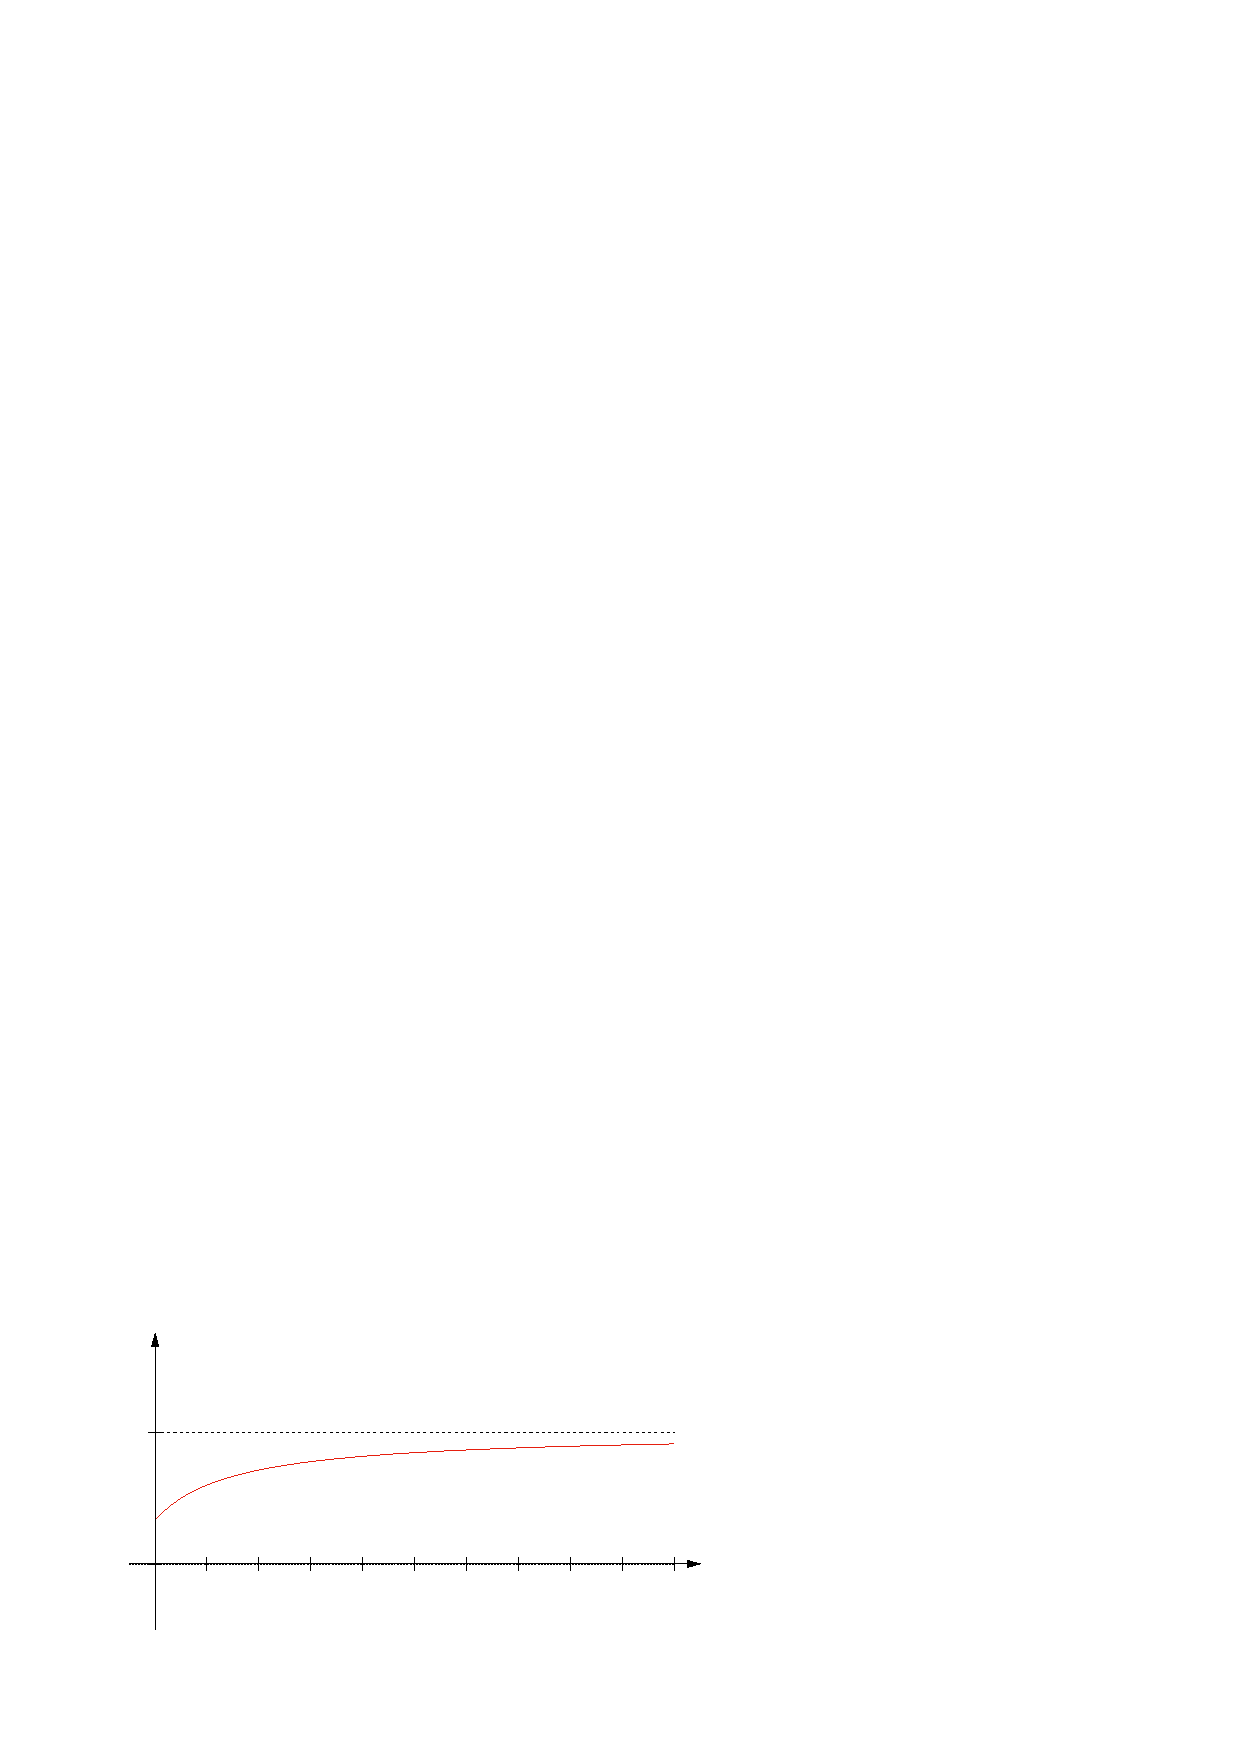
\includegraphics[width={288.00bp},height={144.00bp}]{figura_06_01}}%
    \gplfronttext
  \end{picture}%
\endgroup

\end{figure}

\subsection{Teorema del valor inicial}
Si $\mathcal{L}\{f(t)\}=F(s)$:

\begin{equation}
    f(0)=\lim_{t\rightarrow{0}}f(t)=\lim_{t\rightarrow\infty}sF(s)
\end{equation}

\underline{Prueba}:

\begin{equation*}
    \mathcal{L}\{f'(t)\}=sF(s)-f(0)
\end{equation*}
\begin{equation*}
    \int_0^{\infty}f'(t)\,e^{-st}\,dt=sF(s)-f(0)
\end{equation*}
\begin{equation*}
    \lim_{s\rightarrow\infty}\int_0^{\infty}f'(t)\,e^{-st}\,dt
        =\lim_{s\rightarrow\infty}(sF(s)-f(0))
\end{equation*}
\begin{equation*}
    0=\lim_{s\rightarrow\infty}(sF(s)-f(0))
\end{equation*}
\begin{equation*}
    f(0)=\lim_{s\rightarrow\infty}sF(s)
\end{equation*}

\subsection{Teorema del valor final}
Si $\mathcal{L}\{f(t)\}=F(s)$:

\begin{equation}
    f(\infty)=\lim_{t\rightarrow\infty}f(t)=\lim_{t\rightarrow{0}}sF(s)
\end{equation}

\underline{Prueba}:

\begin{equation*}
    \mathcal{L}\{f'(t)\}=sF(s)-f(0)
\end{equation*}
\begin{equation*}
    \int_0^{\infty}f'(t)\,e^{-st}\,dt=sF(s)-f(0)
\end{equation*}
\begin{equation*}
    \lim_{s\rightarrow{0}}\int_0^{\infty}f'(t)\,e^{-st}\,dt
        =\lim_{s\rightarrow{0}}(sF(s)-f(0))
\end{equation*}
\begin{equation*}
    f(t)\Biggr|_0^{\infty}=\lim_{s\rightarrow{0}}(sF(s)-f(0))
\end{equation*}
\begin{equation*}
    f(\infty)-f(0)=\lim_{s\rightarrow{0}}sF(s)-f(0)
\end{equation*}
\begin{equation*}
    f(\infty)=\lim_{s\rightarrow{0}}sF(s)
\end{equation*}

